% Neural network diagram
% Made with Xematics. Positions are in px (1 px = 0.75 pt), as in the SVG export.
\documentclass[tikz, border=4pt]{standalone}
\definecolor{xm1}{HTML}{FFFFFF}
\definecolor{xm2}{HTML}{F1F2F4}
\definecolor{xm3}{HTML}{4B5563}
\definecolor{xm4}{HTML}{FBE8C4}
\definecolor{xm5}{HTML}{B97800}
\definecolor{xm6}{HTML}{B8C0CC}
\definecolor{xm7}{HTML}{D4E8F5}
\definecolor{xm8}{HTML}{0072B2}
\definecolor{xm9}{HTML}{DFE3E8}
\definecolor{xm10}{HTML}{AEB3B9}
\definecolor{xm11}{HTML}{6B7280}
\definecolor{xm12}{HTML}{1F2937}
\begin{document}
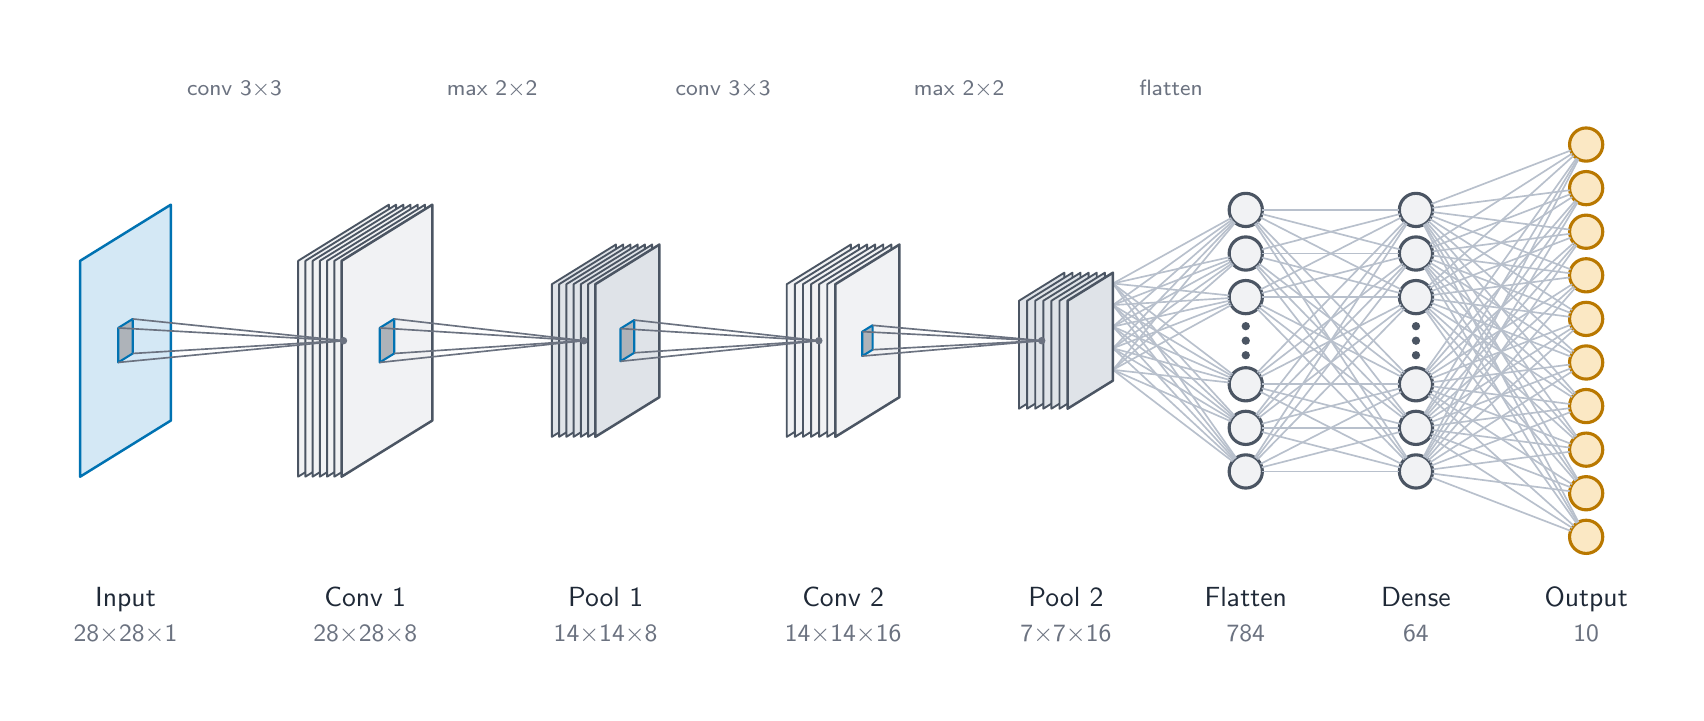
\begin{tikzpicture}[x=0.75pt, y=-0.75pt]
  \tikzset{
    xm hidden/.style={circle, minimum size=12pt, inner sep=0, outer sep=0, fill=xm2, draw=xm3, line width=1.13pt},
    xm output/.style={circle, minimum size=12pt, inner sep=0, outer sep=0, fill=xm4, draw=xm5, line width=1.13pt},
    xm edge/.style={draw=xm6, line width=0.6pt},
    xm map input/.style={fill=xm7, draw=xm8, line width=0.9pt, line join=round},
    xm map hidden back/.style={fill=xm2, draw=xm3, line width=0.68pt, line join=round},
    xm map hidden/.style={fill=xm2, draw=xm3, line width=0.9pt, line join=round},
    xm map pool back/.style={fill=xm9, draw=xm3, line width=0.68pt, line join=round},
    xm map pool/.style={fill=xm9, draw=xm3, line width=0.9pt, line join=round},
    xm dots/.style={fill=xm3},
    xm window/.style={fill=xm10, draw=xm8, line width=0.75pt, line join=round},
    xm ray/.style={draw=xm11, line width=0.6pt},
    xm ray end/.style={fill=xm11},
    xm name xm12/.style={text=xm12, inner sep=0, font=\sffamily\fontsize{9.75}{11.7}\selectfont},
    xm size xm11/.style={text=xm11, inner sep=0, font=\sffamily\fontsize{9}{10.8}\selectfont},
    xm op xm11/.style={text=xm11, inner sep=0, font=\sffamily\fontsize{8.25}{9.9}\selectfont},
  }
  \fill[xm1] (0,0) rectangle (794.11,320.56);
  % Neurons
  \node[xm hidden] (n-5-0) at (586.87,87.81) {};
  \node[xm hidden] (n-5-1) at (586.87,108.81) {};
  \node[xm hidden] (n-5-2) at (586.87,129.81) {};
  \node[xm hidden] (n-5-781) at (586.87,171.81) {};
  \node[xm hidden] (n-5-782) at (586.87,192.81) {};
  \node[xm hidden] (n-5-783) at (586.87,213.81) {};
  \node[xm hidden] (n-6-0) at (668.87,87.81) {};
  \node[xm hidden] (n-6-1) at (668.87,108.81) {};
  \node[xm hidden] (n-6-2) at (668.87,129.81) {};
  \node[xm hidden] (n-6-61) at (668.87,171.81) {};
  \node[xm hidden] (n-6-62) at (668.87,192.81) {};
  \node[xm hidden] (n-6-63) at (668.87,213.81) {};
  \node[xm output] (n-7-0) at (750.87,56.31) {};
  \node[xm output] (n-7-1) at (750.87,77.31) {};
  \node[xm output] (n-7-2) at (750.87,98.31) {};
  \node[xm output] (n-7-3) at (750.87,119.31) {};
  \node[xm output] (n-7-4) at (750.87,140.31) {};
  \node[xm output] (n-7-5) at (750.87,161.31) {};
  \node[xm output] (n-7-6) at (750.87,182.31) {};
  \node[xm output] (n-7-7) at (750.87,203.31) {};
  \node[xm output] (n-7-8) at (750.87,224.31) {};
  \node[xm output] (n-7-9) at (750.87,245.31) {};
  % Connections 4
  \draw[xm edge] (522.87,123.25) -- (n-5-0);
  \draw[xm edge] (522.87,123.25) -- (n-5-1);
  \draw[xm edge] (522.87,123.25) -- (n-5-2);
  \draw[xm edge] (522.87,123.25) -- (n-5-781);
  \draw[xm edge] (522.87,123.25) -- (n-5-782);
  \draw[xm edge] (522.87,123.25) -- (n-5-783);
  \draw[xm edge] (522.87,133.65) -- (n-5-0);
  \draw[xm edge] (522.87,133.65) -- (n-5-1);
  \draw[xm edge] (522.87,133.65) -- (n-5-2);
  \draw[xm edge] (522.87,133.65) -- (n-5-781);
  \draw[xm edge] (522.87,133.65) -- (n-5-782);
  \draw[xm edge] (522.87,133.65) -- (n-5-783);
  \draw[xm edge] (522.87,144.05) -- (n-5-0);
  \draw[xm edge] (522.87,144.05) -- (n-5-1);
  \draw[xm edge] (522.87,144.05) -- (n-5-2);
  \draw[xm edge] (522.87,144.05) -- (n-5-781);
  \draw[xm edge] (522.87,144.05) -- (n-5-782);
  \draw[xm edge] (522.87,144.05) -- (n-5-783);
  \draw[xm edge] (522.87,154.45) -- (n-5-0);
  \draw[xm edge] (522.87,154.45) -- (n-5-1);
  \draw[xm edge] (522.87,154.45) -- (n-5-2);
  \draw[xm edge] (522.87,154.45) -- (n-5-781);
  \draw[xm edge] (522.87,154.45) -- (n-5-782);
  \draw[xm edge] (522.87,154.45) -- (n-5-783);
  \draw[xm edge] (522.87,164.85) -- (n-5-0);
  \draw[xm edge] (522.87,164.85) -- (n-5-1);
  \draw[xm edge] (522.87,164.85) -- (n-5-2);
  \draw[xm edge] (522.87,164.85) -- (n-5-781);
  \draw[xm edge] (522.87,164.85) -- (n-5-782);
  \draw[xm edge] (522.87,164.85) -- (n-5-783);
  % Connections 5
  \draw[xm edge] (n-5-0) -- (n-6-0);
  \draw[xm edge] (n-5-0) -- (n-6-1);
  \draw[xm edge] (n-5-0) -- (n-6-2);
  \draw[xm edge] (n-5-0) -- (n-6-61);
  \draw[xm edge] (n-5-0) -- (n-6-62);
  \draw[xm edge] (n-5-0) -- (n-6-63);
  \draw[xm edge] (n-5-1) -- (n-6-0);
  \draw[xm edge] (n-5-1) -- (n-6-1);
  \draw[xm edge] (n-5-1) -- (n-6-2);
  \draw[xm edge] (n-5-1) -- (n-6-61);
  \draw[xm edge] (n-5-1) -- (n-6-62);
  \draw[xm edge] (n-5-1) -- (n-6-63);
  \draw[xm edge] (n-5-2) -- (n-6-0);
  \draw[xm edge] (n-5-2) -- (n-6-1);
  \draw[xm edge] (n-5-2) -- (n-6-2);
  \draw[xm edge] (n-5-2) -- (n-6-61);
  \draw[xm edge] (n-5-2) -- (n-6-62);
  \draw[xm edge] (n-5-2) -- (n-6-63);
  \draw[xm edge] (n-5-781) -- (n-6-0);
  \draw[xm edge] (n-5-781) -- (n-6-1);
  \draw[xm edge] (n-5-781) -- (n-6-2);
  \draw[xm edge] (n-5-781) -- (n-6-61);
  \draw[xm edge] (n-5-781) -- (n-6-62);
  \draw[xm edge] (n-5-781) -- (n-6-63);
  \draw[xm edge] (n-5-782) -- (n-6-0);
  \draw[xm edge] (n-5-782) -- (n-6-1);
  \draw[xm edge] (n-5-782) -- (n-6-2);
  \draw[xm edge] (n-5-782) -- (n-6-61);
  \draw[xm edge] (n-5-782) -- (n-6-62);
  \draw[xm edge] (n-5-782) -- (n-6-63);
  \draw[xm edge] (n-5-783) -- (n-6-0);
  \draw[xm edge] (n-5-783) -- (n-6-1);
  \draw[xm edge] (n-5-783) -- (n-6-2);
  \draw[xm edge] (n-5-783) -- (n-6-61);
  \draw[xm edge] (n-5-783) -- (n-6-62);
  \draw[xm edge] (n-5-783) -- (n-6-63);
  % Connections 6
  \draw[xm edge] (n-6-0) -- (n-7-0);
  \draw[xm edge] (n-6-0) -- (n-7-1);
  \draw[xm edge] (n-6-0) -- (n-7-2);
  \draw[xm edge] (n-6-0) -- (n-7-3);
  \draw[xm edge] (n-6-0) -- (n-7-4);
  \draw[xm edge] (n-6-0) -- (n-7-5);
  \draw[xm edge] (n-6-0) -- (n-7-6);
  \draw[xm edge] (n-6-0) -- (n-7-7);
  \draw[xm edge] (n-6-0) -- (n-7-8);
  \draw[xm edge] (n-6-0) -- (n-7-9);
  \draw[xm edge] (n-6-1) -- (n-7-0);
  \draw[xm edge] (n-6-1) -- (n-7-1);
  \draw[xm edge] (n-6-1) -- (n-7-2);
  \draw[xm edge] (n-6-1) -- (n-7-3);
  \draw[xm edge] (n-6-1) -- (n-7-4);
  \draw[xm edge] (n-6-1) -- (n-7-5);
  \draw[xm edge] (n-6-1) -- (n-7-6);
  \draw[xm edge] (n-6-1) -- (n-7-7);
  \draw[xm edge] (n-6-1) -- (n-7-8);
  \draw[xm edge] (n-6-1) -- (n-7-9);
  \draw[xm edge] (n-6-2) -- (n-7-0);
  \draw[xm edge] (n-6-2) -- (n-7-1);
  \draw[xm edge] (n-6-2) -- (n-7-2);
  \draw[xm edge] (n-6-2) -- (n-7-3);
  \draw[xm edge] (n-6-2) -- (n-7-4);
  \draw[xm edge] (n-6-2) -- (n-7-5);
  \draw[xm edge] (n-6-2) -- (n-7-6);
  \draw[xm edge] (n-6-2) -- (n-7-7);
  \draw[xm edge] (n-6-2) -- (n-7-8);
  \draw[xm edge] (n-6-2) -- (n-7-9);
  \draw[xm edge] (n-6-61) -- (n-7-0);
  \draw[xm edge] (n-6-61) -- (n-7-1);
  \draw[xm edge] (n-6-61) -- (n-7-2);
  \draw[xm edge] (n-6-61) -- (n-7-3);
  \draw[xm edge] (n-6-61) -- (n-7-4);
  \draw[xm edge] (n-6-61) -- (n-7-5);
  \draw[xm edge] (n-6-61) -- (n-7-6);
  \draw[xm edge] (n-6-61) -- (n-7-7);
  \draw[xm edge] (n-6-61) -- (n-7-8);
  \draw[xm edge] (n-6-61) -- (n-7-9);
  \draw[xm edge] (n-6-62) -- (n-7-0);
  \draw[xm edge] (n-6-62) -- (n-7-1);
  \draw[xm edge] (n-6-62) -- (n-7-2);
  \draw[xm edge] (n-6-62) -- (n-7-3);
  \draw[xm edge] (n-6-62) -- (n-7-4);
  \draw[xm edge] (n-6-62) -- (n-7-5);
  \draw[xm edge] (n-6-62) -- (n-7-6);
  \draw[xm edge] (n-6-62) -- (n-7-7);
  \draw[xm edge] (n-6-62) -- (n-7-8);
  \draw[xm edge] (n-6-62) -- (n-7-9);
  \draw[xm edge] (n-6-63) -- (n-7-0);
  \draw[xm edge] (n-6-63) -- (n-7-1);
  \draw[xm edge] (n-6-63) -- (n-7-2);
  \draw[xm edge] (n-6-63) -- (n-7-3);
  \draw[xm edge] (n-6-63) -- (n-7-4);
  \draw[xm edge] (n-6-63) -- (n-7-5);
  \draw[xm edge] (n-6-63) -- (n-7-6);
  \draw[xm edge] (n-6-63) -- (n-7-7);
  \draw[xm edge] (n-6-63) -- (n-7-8);
  \draw[xm edge] (n-6-63) -- (n-7-9);
  % Layers
  \draw[xm map input] (25.28,112.33) -- (68.96,85.29) -- (68.96,189.29) -- (25.28,216.33) -- cycle;
  \draw[xm map hidden back] (130.32,112.33) -- (174,85.29) -- (174,189.29) -- (130.32,216.33) -- cycle;
  \draw[xm map hidden back] (133.81,112.33) -- (177.49,85.29) -- (177.49,189.29) -- (133.81,216.33) -- cycle;
  \draw[xm map hidden back] (137.3,112.33) -- (180.98,85.29) -- (180.98,189.29) -- (137.3,216.33) -- cycle;
  \draw[xm map hidden back] (140.79,112.33) -- (184.47,85.29) -- (184.47,189.29) -- (140.79,216.33) -- cycle;
  \draw[xm map hidden back] (144.28,112.33) -- (187.96,85.29) -- (187.96,189.29) -- (144.28,216.33) -- cycle;
  \draw[xm map hidden back] (147.77,112.33) -- (191.45,85.29) -- (191.45,189.29) -- (147.77,216.33) -- cycle;
  \draw[xm map hidden] (151.26,112.33) -- (194.94,85.29) -- (194.94,189.29) -- (151.26,216.33) -- cycle;
  \draw[xm map pool back] (252.55,123.6) -- (283.43,104.48) -- (283.43,178.02) -- (252.55,197.14) -- cycle;
  \draw[xm map pool back] (256.04,123.6) -- (286.92,104.48) -- (286.92,178.02) -- (256.04,197.14) -- cycle;
  \draw[xm map pool back] (259.53,123.6) -- (290.41,104.48) -- (290.41,178.02) -- (259.53,197.14) -- cycle;
  \draw[xm map pool back] (263.02,123.6) -- (293.9,104.48) -- (293.9,178.02) -- (263.02,197.14) -- cycle;
  \draw[xm map pool back] (266.51,123.6) -- (297.39,104.48) -- (297.39,178.02) -- (266.51,197.14) -- cycle;
  \draw[xm map pool back] (270,123.6) -- (300.88,104.48) -- (300.88,178.02) -- (270,197.14) -- cycle;
  \draw[xm map pool] (273.49,123.6) -- (304.37,104.48) -- (304.37,178.02) -- (273.49,197.14) -- cycle;
  \draw[xm map hidden back] (365.73,123.6) -- (396.62,104.48) -- (396.62,178.02) -- (365.73,197.14) -- cycle;
  \draw[xm map hidden back] (369.63,123.6) -- (400.52,104.48) -- (400.52,178.02) -- (369.63,197.14) -- cycle;
  \draw[xm map hidden back] (373.53,123.6) -- (404.42,104.48) -- (404.42,178.02) -- (373.53,197.14) -- cycle;
  \draw[xm map hidden back] (377.43,123.6) -- (408.32,104.48) -- (408.32,178.02) -- (377.43,197.14) -- cycle;
  \draw[xm map hidden back] (381.33,123.6) -- (412.22,104.48) -- (412.22,178.02) -- (381.33,197.14) -- cycle;
  \draw[xm map hidden back] (385.23,123.6) -- (416.12,104.48) -- (416.12,178.02) -- (385.23,197.14) -- cycle;
  \draw[xm map hidden] (389.13,123.6) -- (420.02,104.48) -- (420.02,178.02) -- (389.13,197.14) -- cycle;
  \draw[xm map pool back] (477.63,131.57) -- (499.47,118.05) -- (499.47,170.05) -- (477.63,183.57) -- cycle;
  \draw[xm map pool back] (481.53,131.57) -- (503.37,118.05) -- (503.37,170.05) -- (481.53,183.57) -- cycle;
  \draw[xm map pool back] (485.43,131.57) -- (507.27,118.05) -- (507.27,170.05) -- (485.43,183.57) -- cycle;
  \draw[xm map pool back] (489.33,131.57) -- (511.17,118.05) -- (511.17,170.05) -- (489.33,183.57) -- cycle;
  \draw[xm map pool back] (493.23,131.57) -- (515.07,118.05) -- (515.07,170.05) -- (493.23,183.57) -- cycle;
  \draw[xm map pool back] (497.13,131.57) -- (518.97,118.05) -- (518.97,170.05) -- (497.13,183.57) -- cycle;
  \draw[xm map pool] (501.03,131.57) -- (522.87,118.05) -- (522.87,170.05) -- (501.03,183.57) -- cycle;
  \fill[xm dots] (586.87,143.81) circle[radius=2];
  \fill[xm dots] (586.87,150.81) circle[radius=2];
  \fill[xm dots] (586.87,157.81) circle[radius=2];
  \fill[xm dots] (668.87,143.81) circle[radius=2];
  \fill[xm dots] (668.87,150.81) circle[radius=2];
  \fill[xm dots] (668.87,157.81) circle[radius=2];
  \draw[xm window] (43.63,144.65) -- (50.62,140.33) -- (50.62,156.97) -- (43.63,161.29) -- cycle;
  \draw[xm ray] (43.63,144.65) -- (152.16,150.81);
  \draw[xm ray] (50.62,140.33) -- (152.16,150.81);
  \draw[xm ray] (50.62,156.97) -- (152.16,150.81);
  \draw[xm ray] (43.63,161.29) -- (152.16,150.81);
  \fill[xm ray end] (152.16,150.81) circle[radius=1.8];
  \draw[xm window] (169.61,144.65) -- (176.6,140.33) -- (176.6,156.97) -- (169.61,161.29) -- cycle;
  \draw[xm ray] (169.61,144.65) -- (267.99,150.81);
  \draw[xm ray] (176.6,140.33) -- (267.99,150.81);
  \draw[xm ray] (176.6,156.97) -- (267.99,150.81);
  \draw[xm ray] (169.61,161.29) -- (267.99,150.81);
  \fill[xm ray end] (267.99,150.81) circle[radius=1.8];
  \draw[xm window] (285.62,144.98) -- (292.24,140.88) -- (292.24,156.64) -- (285.62,160.74) -- cycle;
  \draw[xm ray] (285.62,144.98) -- (381.18,150.81);
  \draw[xm ray] (292.24,140.88) -- (381.18,150.81);
  \draw[xm ray] (292.24,156.64) -- (381.18,150.81);
  \draw[xm ray] (285.62,160.74) -- (381.18,150.81);
  \fill[xm ray end] (381.18,150.81) circle[radius=1.8];
  \draw[xm window] (402.11,146.46) -- (407.05,143.4) -- (407.05,155.16) -- (402.11,158.22) -- cycle;
  \draw[xm ray] (402.11,146.46) -- (488.55,150.81);
  \draw[xm ray] (407.05,143.4) -- (488.55,150.81);
  \draw[xm ray] (407.05,155.16) -- (488.55,150.81);
  \draw[xm ray] (402.11,158.22) -- (488.55,150.81);
  \fill[xm ray end] (488.55,150.81) circle[radius=1.8];
  % Labels
  \node[xm name xm12, anchor=base] at (47.12,278.9) {Input};
  \node[xm size xm11, anchor=base] at (47.12,295.66) {28\ensuremath{\times}28\ensuremath{\times}1};
  \node[xm op xm11, anchor=base] at (99.64,32.66) {conv 3\ensuremath{\times}3};
  \node[xm name xm12, anchor=base] at (162.63,278.9) {Conv 1};
  \node[xm size xm11, anchor=base] at (162.63,295.66) {28\ensuremath{\times}28\ensuremath{\times}8};
  \node[xm op xm11, anchor=base] at (223.75,32.66) {max 2\ensuremath{\times}2};
  \node[xm name xm12, anchor=base] at (278.46,278.9) {Pool 1};
  \node[xm size xm11, anchor=base] at (278.46,295.66) {14\ensuremath{\times}14\ensuremath{\times}8};
  \node[xm op xm11, anchor=base] at (335.05,32.66) {conv 3\ensuremath{\times}3};
  \node[xm name xm12, anchor=base] at (392.88,278.9) {Conv 2};
  \node[xm size xm11, anchor=base] at (392.88,295.66) {14\ensuremath{\times}14\ensuremath{\times}16};
  \node[xm op xm11, anchor=base] at (448.82,32.66) {max 2\ensuremath{\times}2};
  \node[xm name xm12, anchor=base] at (500.25,278.9) {Pool 2};
  \node[xm size xm11, anchor=base] at (500.25,295.66) {7\ensuremath{\times}7\ensuremath{\times}16};
  \node[xm op xm11, anchor=base] at (550.87,32.66) {flatten};
  \node[xm name xm12, anchor=base] at (586.87,278.9) {Flatten};
  \node[xm size xm11, anchor=base] at (586.87,295.66) {784};
  \node[xm name xm12, anchor=base] at (668.87,278.9) {Dense};
  \node[xm size xm11, anchor=base] at (668.87,295.66) {64};
  \node[xm name xm12, anchor=base] at (750.87,278.9) {Output};
  \node[xm size xm11, anchor=base] at (750.87,295.66) {10};
\end{tikzpicture}
\end{document}
